\section{Study Area and Data}
\label{sec:data}

\subsection{One operator, one number}

Pakistan Railways operates the country's mainline rail network as a state enterprise. Its Year
Book reports fuel consumption by product, traffic by division, and train-kilometres by service
class. The datum is what the source calls it: the table is headed \emph{Fuel Consumption}, and
the narrative states that the quantities ``comprise the entire fuel consumed on the Railways,
i.e.\ on locomotives, power houses, water pumps, workshops etc.'' This inventory adopts the
Tier~1 assumption that fuel consumed in a fiscal year equals fuel burnt in it; no depot-stock
or procurement-timing correction is published, and none is attempted. The reference year here
is FY2023--24: the 2024--25 edition is a page-image scan whose own Legal Opinion page
declares its data provisional pending audit, so its year enters the series flagged
provisional rather than as the reference.

\begin{table}[htbp]
\centering
\footnotesize
\begin{tabular}{@{}lrr@{}}
\toprule
\textbf{Stream} & \textbf{TJ} & \textbf{\% of energy} \\
\midrule
Diesel      & 4817.6 & 99.933 \\
Furnace oil &    3.2 &  0.067 \\
\bottomrule
\end{tabular}
\caption{Railway module fuel, FY2023--24. Diesel is \num{132588} thousand litres---the
metered total, of which \num{1599} thousand litres is the measured non-traction share;
furnace oil is a rounding error carried for the reason given below.}
\label{tab:fuel}
\end{table}

\begin{figure}[htbp]
\centering
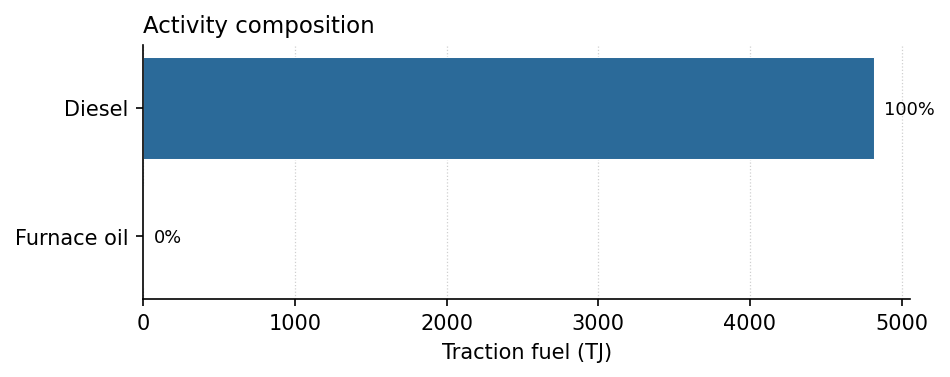
\includegraphics[width=\linewidth]{railways_activity.png}
\caption{The energy basis. One stream is the sector.}
\label{fig:activity}
\end{figure}

\subsection{Electric traction: none since about 2010, and none in scope}

Recent Year Book editions report Electric Energy as NIL, and the historical table behind that
figure says when it became true. Electric traction energy is non-zero from the 1985--90
quinquennium (\SI{37.4}{\giga\watt\hour} per year on average) and declines through 2005--2010
(\SI{6.1}{\giga\watt\hour}) before going NIL from the 2010--2015 row. The Lahore--Khanewal
electrification---the operator's only electrified section---therefore ran into the late
2000s, not the 1970s as this paper previously stated; the mainline network has been
diesel-only since roughly 2010, which covers every inventory year here. The sector
consequently has no scope-2 stream, unlike residential fuel where the electricity boundary has
to be argued.

The scope is the Pakistan Railways mainline system's direct combustion. Urban electric rail
outside the operator---the Lahore Orange Line metro---has zero direct 1A3c combustion
emissions by definition; its electricity-related emissions belong to power generation, and the
boundary is recorded in the completeness assessment rather than left implicit in a NIL row.

\subsection{Two things the source does badly, both recorded}

\textbf{Five editions are scans, and it turned out not to matter.} The 2017--18, 2018--19,
2019--20, 2021--22 and 2024--25 editions are page images with no extractable text layer, and
this paper previously reported FY2018 and FY2019 as absent from the time series for that
reason.

That was true about those editions and wrong about the data. Every edition's fuel table carries
a historical run, not just the current year, and the 2020--21 edition has a text layer: it
reports FY2015--16 through FY2020--21 annually. Both missing years were one edition later the
whole time. They are now in the series---\num{156396} and \num{159927} thousand
litres---recovered rather than interpolated, and the series runs FY2014--FY2025 unbroken.

What makes them trustworthy is that the same table reproduces FY2016, FY2017 and FY2021
exactly against figures this inventory already held from other editions. A test asserts that
correspondence, and a second asserts the series is contiguous, because the honest reason to
leave a hole in it has gone.

\textbf{Furnace oil changed unit labels without announcement, and the source itself settles
the basis.} Editions through 2020--21 label the row ``Tonnes'' and editions from 2022--23 label
it ``Liters/thousand,'' with no note explaining the change. The 2023--24 edition resolves it
against itself: its detailed fuel table and the narrative on the same page state the quantity
in metric tonnes, and the summary table's unit column is demonstrably unreliable
(Section~\ref{sec:limitations}). The basis is tonnes, and that is what the activity file
carries. The stream is under \SI{0.001}{\mega\tonne} \COe{} on either reading, so nothing
material turns on it, and a test pins that indifference by recomputing the total under both
interpretations. The unit travels with each row in the activity file rather than being
inferred from the year, so any future correction is a data edit and not a code change.

Furnace oil is carried at all for two reasons: IPCC Chapter~3 §3.4.1.4 warns specifically
against omitting non-diesel traction fuels, and an unexplained unit change in a government
series is worth recording where the next person will find it.

\subsection{The traffic statistics}

The same Year Book reports \num{26885} thousand passenger, mixed and other coaching
train-kilometres and \num{6237} thousand freight, \num{33122} thousand in total. These do not
enter the estimate. They are carried as a parameter because they permit the fuel figure to be
checked against the traffic that consumed it, which is the evidence behind
Section~\ref{sec:validation}.
